
\section{Making Modeling Choices}
\label{sec:modeling-choices}

\subsection{Computational box} \label{subsect:coords}
\optsection{Computational box}
\optseealso{Grid}

PISM does all simulations in a computational box\index{PISM!computational box} which is rectangular in the PISM coordinates.

The coordinate system has horizontal coordinates $x,y$ and a vertical coordinate $z$.  The $z$ coordinate is measured positive upward from the base of the ice and it is exactly opposite to the vector of gravity.  The surface $z=0$ is the base of the ice, however, and thus is usually not horizontal in the sense of being parallel to the geoid.   The surface $z=0$ is the base of the ice both when the ice is grounded and when the ice is floating.

Bed topography is, of course, allowed.  In fact, when the ice is grounded, the true physical vertical coordinate $z'$, namely the coordinate measure relative to a reference geoid, is given by $z'=z+b(x,y)$ where $b(x,y)$ is the bed topography.  The surface $z'=h(x,y)$ is the surface of the ice.

In the grounded case the equation $h(x,y)=H(x,y)+b(x,y)$ always applies if $H(x,y)$ is the thickness of the ice.  In the floating case, the physical vertical coordinate is $z'=z-(\rho_i/\rho_s) H(x,y)$ where $\rho_i$ is the density of ice and $\rho_s$ the density of sea water.  Again $z=0$ is the base of the ice, which is the surface $z' = -(\rho_i/\rho_s) H(x,y)$.  The surface of the ice is $h(x,y) = (1-\rho_i/\rho_s) H(x,y)$.  All we know about the bed elevations is that they are below the base of the ice when the ice is floating.  That is, the \emph{flotation criterion} $-(\rho_i/\rho_s) H(x,y) > b(x,y)$ applies.

The computational box can extend downward into the bedrock.  As $z=0$ is the base of the ice, the bedrock corresponds to negative $z$ values regardless of the sign of its true (i.e.~$z'$) elevation.

The extent of the computational box, along with its bedrock extension downward, is determined by four numbers \texttt{Lx}, \texttt{Ly}, \texttt{Lz}, and \texttt{Lbz} (see Figure \ref{fig:rectilinearbox}.).  The first two of these are half-widths and have units of kilometers when set by options or displayed.  The extent of the computational box for the ice and bedrock is directly controlled by the following options. 

\begin{center}
  \begin{tabular}{llp{0.7\linewidth}}
    \toprule
    \textbf{Option} & \textbf{Meaning}
    \\\midrule
    \txtopt{Lx}{(km)} & Half-width of the computational domain (in the $x$-direction) \\
    \txtopt{Ly}{(km)} & Half-width of the computational domain (in the $y$-direction) \\
    \txtopt{Lz}{(meters)} & Height of the computational domain in the ice \\
    \txtopt{Lbz}{(meters)} & Depth of the computational domain in the bedrock thermal layer
    \\\bottomrule
  \end{tabular}
\end{center}

\begin{figure}[ht]
\centering
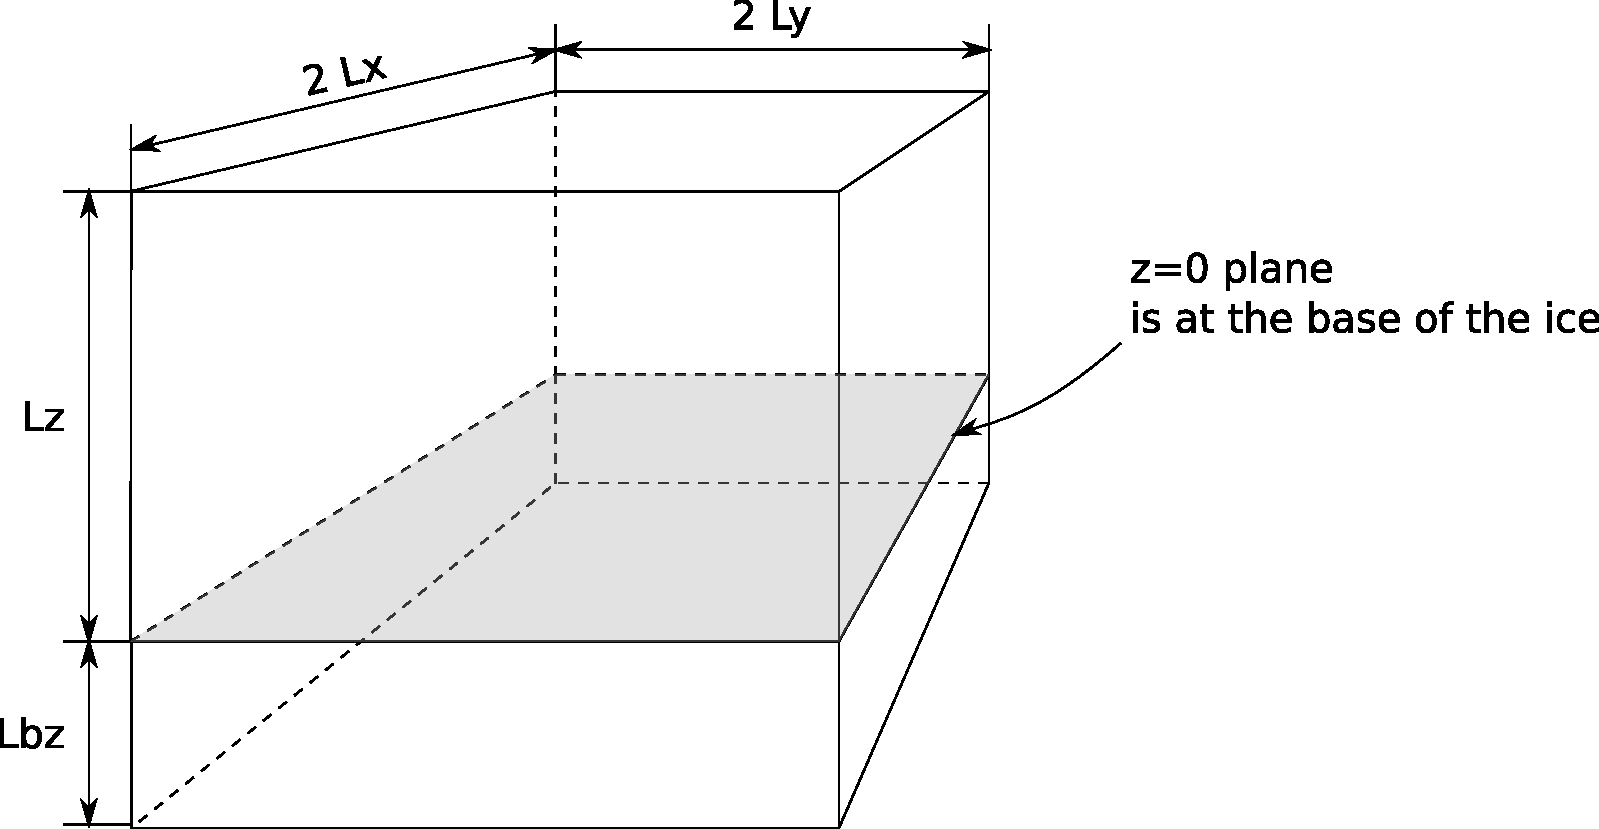
\includegraphics[width=4.0in,keepaspectratio=true]{rectilinearbox}
\caption{PISM's computational box.}
\label{fig:rectilinearbox}
\end{figure}


\subsection{Spatial grid}
\label{subsect:grid}
\optsection{Grid!space}

The PISM grid\index{PISM!grid} covering the computational box is equally spaced in horizontal ($x$ and $y$) directions.  Vertical spacing in the ice is quadratic by default (see below) but optionally a different spacing scheme can be chosen.  (Choose with options \txtopt{z_spacing}{[quadratic, equal]}.) The bedrock thermal layer model always uses equal vertical spacing.

The grid is described by four numbers, namely the number of grid points \texttt{Mx} in the $x$ direction, the number \texttt{My} in the $y$ direction, the number \texttt{Mz} in the $z$ direction within the ice, and the number \texttt{Mbz} in the $z$ direction within the bedrock thermal layer.  These are specified by options \intextoption{Mx}, \intextoption{My}, \intextoption{Mz}, and \intextoption{Mbz}, respectively. The defaults are 61, 61, 31, and 1, respectively.

Note that \texttt{Mx}, \texttt{My}, \texttt{Mz}, and \texttt{Mbz} all indicate the number of grid \emph{points}.  The numbers of grid \emph{spaces} are one less, thus 60, 60, 30, and 0 in the default case.  The lowest grid point in a column of ice, at $z=0$, coincides with the highest grid point in the bedrock, so \texttt{Mbz} must always be at least one and \texttt{Mbz}$>1$ is required to use the bedrock thermal model.  Note that this option is unrelated to the bed deformation model (glacial isostasy model); see option \texttt{-bed_def} (section \ref{subsect:beddef}) for that.

In the quadratic case, the spacing near the ice/bedrock interface is about four times finer than it would be with equal spacing for the same value of \texttt{Mz}, while the spacing near the top is correspondingly coarser. For a detailed description of the spacing of the grid, see the documentation on \texttt{IceGrid::compute_vertical_levels()} in the PISM class browser.

When a thermal bedrock layer is used, the distance \texttt{Lbz} is controlled by the \texttt{-Lbz} option.

If one initializes PISM from a saved model state using \texttt{-i} then the input model state controls all computational grid parameters.  For instance, the command

\begin{verbatim}
$  pismr -i foo.nc -y 100
\end{verbatim}

\noindent should work fine if \texttt{foo.nc} was a valid PISM model file.  The command

\begin{verbatim}
$  pismr -i foo.nc -Mz 201 -y 100
\end{verbatim}

\noindent will give a warning that ``\texttt{PISM WARNING: ignoring command-line option '-Mz'}'' because \texttt{-i} input files take precedence.

Otherwise, one is allowed to specify the grid when PISM is started.  In particular, the user should specify the grid when using \texttt{-boot_file} or when initializing a simplified-geometry experiment or a verification test, though defaults are generally present in the latter cases.  See sections \ref{sec:start} and \ref{sec:boot} for examples and explanation.


\subsection{Model time}
\label{sec:time}
\optsection{Grid!time}

The following command-line options control PISM time:

\begin{tabular}{lp{0.8\linewidth}}\\
\toprule
\textbf{Option} & \textbf{Meaning}\\
\midrule
\txtopt{y}{(years)} & Number of model years to run.\\
\txtopt{ys}{(years)} & Model year at which to start the run.  Also resets the model time, ignoring any time in the input file.\\
\txtopt{ye}{(years)} & Model year at which to end the run.\\
\bottomrule
\end{tabular}
\\[2em]
\noindent The default value for the end year is the start year (\texttt{-ys} or initialized model time from file) plus the default or given (\texttt{-y}) run length.  If both \texttt{-ys} and \texttt{-ye} are used then the run length is set to the difference.  Using all three of \texttt{-ys}, \texttt{-y} and \texttt{-ys} is not allowed.

Most of PISM (and its ice dynamics core in particular) only needs to know the length of the current time-step. This explains the unsophisticated interface described here. Careful application of climate data and model validation requires well-organized management of model time, though. Please see the \emph{PISM's climate forcing components} manual for an alternative, calendar-aware, time-management interface.

\subsection{Diagnostic computations}
\label{sec:diagnostic-computations}

 As a diagnostic example, consider the second of these two runs:
\begin{verbatim}
pisms -y 6000 -o foo.nc
pismr -i foo.nc -y 0 -o bar.nc -o_size big
\end{verbatim}

\noindent The result of this zero-length, ``\texttt{-y 0}'', run is a NetCDF file \texttt{bar.nc} which contains the full three-dimensional velocity field in the scalar NetCDF variables \texttt{uvel}, \texttt{vvel}, and \texttt{wvel}, as well as many other variables.  The file \texttt{foo.nc} does not contain many of these fields because it was written with the default output size of \texttt{medium}.  The ``\texttt{-y 0}'' run has diagnostically ``filled-in'' the fields which PISM can model at a time step, but the model state has not evolved.

In fact, during such a run PISM performs one short time-step to compute ``rates of change'' of ice thickness, surface elevation and other fields, but the model state \emph{is reset} after this step, so re-starting from \texttt{foo.nc} above would give the same result as re-starting from \texttt{bar.nc}.

This diagnostic mode is most frequently associated to the modeling of ice shelves and ice streams.  Subsection \ref{sec:ross} describes using \texttt{pross} to model the Ross ice shelf \cite{MacAyealetal}.  Verification tests I and J, section \ref{sec:verif}, are diagnostic calculations using the SSA.

Note that the NetCDF model state saved by PISM at the end of an \emph{evolution} run does not, by default, contain the three-dimensional velocity field.  Instead, it contains just a bit more than the variables which are needed to restart the run.  One can  force PISM to save all the supported diagnostic quantities at the end of a time-stepping run using the option \texttt{-o_size big}.  Or one can go back and do a ``\texttt{-y 0}'' diagnostic run.


\subsection{Computing ice age} \label{subsect:age}
\optsection{Computing ice age}

By default, PISM does not compute the age of the ice\index{PISM!modeling the age of the ice} because it does not directly impact ice flow when using the default flow laws. It is very easy to turn on.  Just set \intextoption{age}.

  
\subsection{Flotation criterion and mask} \label{subsect:floatmask}  The most basic decision about ice dynamics made internally by PISM is whether to apply the ``flotation criterion'' to determine whether the ice is floating on the ocean or not.  In an evolution run this decision is made at each time step and the result is stored in the \texttt{mask}.

The possible values of the \texttt{mask}\index{mask} are given in Table \ref{tab:maskvals}.  The mask does not by itself determine ice dynamics.  For instance, when ice is floating (either value \texttt{MASK_FLOATING} or \texttt{MASK_FLOATING_AT_TIME_0}) the usual choice for ice dynamics is SSA, but the user can choose not to apply that model by not using either option \texttt{-ssa_floating_only} or \texttt{-ssa_sliding}.

\begin{table}[ht]
  \centering
 \small
  \begin{tabular}{p{0.25\linewidth}p{0.65\linewidth}}
    \toprule
    \textbf{Mask value} & \textbf{Meaning}\\
    \midrule
    -1=\texttt{MASK_UNKNOWN} & not set, does not appear in PISM output files \\
    0=\texttt{MASK_ICE_FREE_BEDROCK} & ice free bedrock \\
    2=\texttt{MASK_GROUNDED}& ice is grounded (and the SIA is always applied, while the SSA is also applied if \texttt{-ssa_sliding} is given) \\
    3=\texttt{MASK_FLOATING} & ice is floating (and the SSA is applied if one of \texttt{-ssa_sliding} or \texttt{-ssa_floating_only} is given) \\
    4=\texttt{MASK_ICE_FREE_OCEAN} & ice-free ocean \\
    \\\bottomrule
  \end{tabular}
  \normalsize
  \caption{The PISM mask\index{mask}, in combination with user options, determines the dynamical model.}
  \label{tab:maskvals} 
\end{table}

Assuming the geometry of the ice evolves (which can be turned off by option \texttt{-no_mass}), and assuming an ocean exists (which can be turned off by option \texttt{-dry}), then at each time step the mask changes by the flotation criterion.  Ice which becomes floating is marked as \texttt{MASK_FLOATING} while ice which becomes grounded is marked as \texttt{MASK_GROUNDED}.

\subsection{Rheology}
\label{sec:rheology}
\optsection{Rheology}

In the polythermal (default) mode of PISM there is only one choice of the flow law: the Glen-Paterson-Budd-Lliboutry-Duval \cite{AschwandenBlatter,LliboutryDuval1985,PatersonBudd}. This law is the only one which we know of in the literature that parameterizes the (observed) softening of pressure-melting-temperature ice, as its liquid fraction increases.

Note that a ``flow law'' here means the function $F(\sigma,T,\omega,P,d)$ in the relation
	$$\dot \eps_{ij} = F(\sigma,T,\omega,P,d)\, \sigma_{ij}'$$
where $\dot \eps_{ij}$ is the strain rate tensor, $\sigma_{ij}'$ is the stress deviator tensor, $T$ is the ice temperature, $\omega$ is the liquid water fraction in the ice, $\sigma^2 = \frac{1}{2} \|\sigma_{ij}'\|_F$, so $\sigma$ is the second invariant of the stress deviator tensor, $P$ is the pressure, and $d$ is the grain size. For example, $F = A \sigma^{n-1}$ is the isothermal Glen law. That is, we are addressing isotropic flow laws only.  In PISM one can choose the scalar function $F$ reasonably arbitrarily by modifying source code,\footnote{See source files \texttt{flowlaws.hh}, \texttt{flowlaws.cc} in \texttt{src/base/rheology/}.} or use the single polythermal law (above), or choose among a number of ``cold ice'' laws listed in table \ref{tab:flowlaw}.

Note that the inverse form of such a flow law in needed for ice shelves and ice streams:
	$$\sigma_{ij}' = 2 \nu(\dot\eps,T,\omega,P,d)\,\dot \eps_{ij} $$
Here $\nu(\dot \eps,T,\omega,P,d)$ is the effective viscosity.

The command-line options \intextoption{sia_e} and \intextoption{ssa_e} set flow enhancement factors for the SIA and SSA respectively. These options can be used with any flow law.  (The enhancement factor $e$ alters the SIA flow law to be ``$\dot \eps_{ij} = e\, F(\sigma,T,\omega,P,d)\, \sigma_{ij}'.$'')

Command-line options \intextoption{sia_flow_law} and \intextoption{ssa_flow_law} control SIA and SSA the flow laws in the \texttt{-cold} mode.  Allowed arguments are listed in table \ref{tab:flowlaw} below.

Flow law parameters such as ice softness can be changed using configuration parameters (see section \ref{sec:pism-defaults} and the implementation of flow laws in the \emph{Source Code Browser}).

\begin{table}[ht]
\centering
\index{rheology}\index{flow law}
\small
\begin{tabular}{p{0.18\linewidth}p{0.2\linewidth}p{0.52\linewidth}}\toprule
\textbf{Type} & C++ Class & \textbf{Comments and Reference} \\ \midrule
\texttt{pb} &\texttt{ThermoGlenIce}  & Paterson-Budd law, the cold-mode default.  Fixed Glen exponent $n=3$.  There is a split ``Arrhenius'' term $A(T) = A \exp(-Q/RT^*)$ where \mbox{$A = 3.615 \times 10^{-13}\, \text{s}^{-1}\, \text{Pa}^{-3}$}, \mbox{$Q = 6.0 \times 10^4\, \text{J}\, \text{mol}^{-1}$} if $T^* < 263$ K and
 \mbox{$A = 1.733 \times 10^{3}\, \text{s}^{-1}\, \text{Pa}^{-3}$}, \mbox{$Q = 13.9 \times 10^4\, \text{J}\, \text{mol}^{-1}$} if $T^* > 263$ K and where $T^*$ is the pressure-adjusted temperature \cite{PatersonBudd}. \\
\texttt{arr} &  \texttt{ThermoGlenArrIce} & \emph{Cold} part of Paterson-Budd.  Regardless of temperature, the $A$ and $Q$ values for $T^*<263$ K in  the Paterson-Budd law apply.  This is the flow law used in the thermomechanically coupled exact solutions Tests \textbf{F} and \textbf{G} described in \cite{BBL,BB} and run by \texttt{pismv -test F} and \texttt{pismv -test G}. \\
\texttt{arrwarm} & \texttt{ThermoGlenArrIceWarm} & \emph{Warm} part of Paterson-Budd.  Regardless of temperature, the $A$ and $Q$ values for $T^*>263$ K in Paterson-Budd apply.\\
\texttt{hooke} & \texttt{HookeIce} & Hooke law.  Fixed Glen exponent $n=3$.  Here  \mbox{$A(T) = A \exp(-Q/(RT^*) + 3C (T_r - T^*)^\kappa)$;} values of  constants as in \cite{Hooke,PayneBaldwin}.\\
\texttt{gk} & \texttt{GoldsbyKohlstedtIce} & The  Goldsby-Kohlstedt flow law.  This law has a combination of exponents  from $n=1.8$ to $n=4$ \cite{GoldsbyKohlstedt}. It does not have a viscosity form and can only be used by the SIA stress balance. \\
\texttt{isothermal_glen} &  \texttt{IsothermalGlenIce} &The isothermal Glen flow law. \\
\bottomrule
\normalsize	
\end{tabular}
\caption{\emph{For} \texttt{-cold} \emph{mode only:} Choosing the rheology using \texttt{-sia_flow_law} and \texttt{-ssa_flow_law}.}
\label{tab:flowlaw}
\end{table}

\subsection{Choosing the stress balance}  \label{subsect:ssacontrol}
\optsection{SSA as a sliding law}

The basic stress balance used for all grounded ice in PISM is the non-sliding, thermomechanically-coupled SIA \cite{BBL}.  For the vast majority of most ice sheets, as measured by area or volume, this is an appropriate model which is an $O(\eps^2)$ approximation to the Stokes model \cite{Fowler}.

The shallow shelf approximation (SSA)\index{SSA (shallow shelf approximation)} stress balance applies to floating ice.  Option \texttt{-ssa_floating_only} turns on this stress balance but restricted only to floating ice.  See the Ross ice shelf example in section \ref{sec:ross} for an example in which the SSA is only applied to floating ice.

The SSA is also used in PISM to describe the sliding of grounded ice and the formation of ice streams \cite{BBssasliding}.  Specifically for the SSA with ``plastic'' (Coulomb friction) basal resistance, the locations of ice streams are determined as part of a free boundary problem of Schoof \cite{SchoofStream}, a model for emergent ice streams within a ice sheet and ice shelf system.  This model explains ice streams through a combination of plastic till failure and SSA stress balance.  As a combination of SIA and SSA it is a ``hybrid'' approximation of the Stokes model \cite{BBssasliding,Winkelmannetal2011}.  In other words, this SSA description of ice streams is the preferred ``sliding law'' for the SIA, and it should be used in preference to classical SIA sliding laws which make ice basal velocity a local function of the basal value of the driving stress \cite{BBssasliding}.\index{SIA (shallow ice approximation)!sliding laws}

Option \texttt{-ssa_sliding} turns on such use of the plastic till SSA as a sliding law; floating ice is also subject to the SSA with this option.  Of course the is more to the use of a stress balance than just turning it on.  At all grounded points a yield stress, or a pseudo-yield-stress in the case of power law sliding (subsection \ref{subsect:basestrength}), is computed from the amount of stored basal water and from a (generally) spatially-varying till strength.  The amount of stored basal water is modeled by the subglacial hydrology mode choice (subsection \ref{subsect:subhydro}) based on the basal melt rate which is, primarily, thermodynamically-determined (subsection \ref{subsect:basestrength}).

Table \ref{tab:stressbalchoice} describes the basic choice of stress balance, while Table \ref{tab:ssausage} describes additional controls on the numerical solution of the stress balance equations.

\begin{table}[ht]
\centering
\small
\begin{tabular}{p{0.25\linewidth}p{0.65\linewidth}}
\toprule
\textbf{Option} & \textbf{Semantics}\\ \midrule
    (\emph{NO OPTION}) & Grounded ice flows by the non-sliding SIA.  (Floating ice essentially doesn't flow, so this model is not recommended for marine ice sheets.) \\
    \intextoption{ssa_floating_only} & Only floating ice uses SSA.  Grounded ice marked by mask value \texttt{SHEET} uses the (by default) nonsliding SIA. \\
\intextoption{ssa_sliding} & The recommended default sliding law, which gives the SIA+SSA hybrid stress balance.  Combines SSA-computed velocity, using pseudo-plastic till, with SIA-computed velocity according to the combination in \cite{BBssasliding}.  Floating ice uses SSA only. \\
\bottomrule
\end{tabular}
\normalsize
\caption{The basic choice of stress balance.}
\label{tab:stressbalchoice} 
\end{table}


\begin{table}
  \centering
  \begin{tabular}{p{0.22\linewidth}p{0.75\linewidth}}
     \toprule
     \textbf{Option} & \textbf{Description}\\\midrule
     \intextoption{ssa_method} [\texttt{fd}$\big|$\texttt{fem}] & Both finite difference (\texttt{fd}) and finite element (\texttt{fem}) versions of the SSA numerical solver are implemented in PISM.  They behave similarly for runs without PIK options (section \ref{sec:pism-pik}), but the \texttt{fd} solver is the only one which allows PIK options.  \texttt{fd} uses Picard iteration \cite{BBssasliding}, while \texttt{fem} uses a Newton method.  The \texttt{fem} solver has in-development surface velocity inversion capability \cite{Habermannetal2012}.  \\
     \intextoption{ssa_eps} (1.0e13) & The numerical scheme for the SSA computes an effective viscosity $\nu$ which which depends on strain rates and ice hardness (thus on temperature).  The value of, and the minimum of, the effective viscosity times the thickess (i.e.~$\nu H$) is important to ease of solving the numerical SSA.  This constant is added ($\nu H \to \nu H + \text{\texttt{ssa_eps}}$) to keep this quantity bounded away from zero.  The units of \texttt{ssa_eps} are $\text{Pa}\,\text{m}\,\text{s}$.  Turn off this lower bound mechanism by \texttt{-ssa_eps 0.0}.  Use option \texttt{-ssa_view_nuh} to view the product $\nu H$ for your simulation, to evaluate the relative importance of this \texttt{ssa_eps} regularization.  Note that a typical Greenland run might see a wide range of values for $\nu H$ from $\sim 10^{14}$ to $\sim 10^{20}$ $\text{Pa}\,\text{m}\,\text{s}$ for $\nu H$. \\
     \intextoption{ssa_maxi} (300) & (\emph{Only active with} \texttt{-ssa_method fd}, \emph{the default}.)  Set the maximum allowed number of Picard (nonlinear) iterations in solving the shallow shelf approximation.\\
     \intextoption{ssa_rtol} (1.0e-4) & (\emph{Only active with} \texttt{-ssa_method fd}, \emph{the default}.)  The numerical scheme for the SSA does a nonlinear iteration wherein velocities (and temperatures) are used to compute a vertically-averaged effective viscosity which is used to solve the equations for horizontal velocity.  Then the new velocities are used to recompute an effective viscosity, and so on.  This option sets the relative change tolerance for the effective viscosity.
In particular, the nonlinear part of the iteration requires that successive values $\nu^{(k)}$ of the vertically-averaged effective viscosity satisfy
	$\|(\nu^{(k)} - \nu^{(k-1)}) H\|_1 \le \text{\texttt{ssa_rtol}} \|\nu^{(k)} H\|_1$
in order to end the iteration with $\nu = \nu^{(k)}$.  (See also PETSc option \texttt{-ksp_rtol} to control relative tolerance for the iteration inside the linear solver.)\\
\bottomrule
\end{tabular}
\caption{Controlling the numerical SSA stress balance in PISM}
\label{tab:ssausage}
\end{table}


\subsection{Surface gradient method}
\label{subsect:gradient}
\optsection{Driving stress computation}

PISM computes surface gradients to determine the ``driving stress''
	$$(\tau_{d,x},\tau_{d,y}) = - \rho g H \grad h,$$
where $H$ is the ice thickness, and $h = H+b$ is the ice surface elevation.  The driving stress enters into both the SIA and SSA stress balances, but in the former the driving stress is needed on a staggered grid, while in the latter the driving stress is needed on the regular grid.

Surface gradients are computed by finite differences in several slightly-different ways.  There are options for choosing which method to use, but to the best of our knowledge there is no theoretical advice on the best, most robust mechanism.  There are three \intextoption{gradient} methods in PISM:

\noindent\texttt{-gradient mahaffy}\quad  This most ``standard'' way computes the surface slope onto the staggered grid for the SIA \cite{Mahaffy}.  It makes $O(\Delta x^2,\Delta y^2)$ errors.  For computations of driving stress on the regular grid, centered differencing is used instead.

\noindent\texttt{-gradient haseloff}\quad  This is the default method, but it only differs from the Mahaffy method at ice-margin locations.  It alters the \texttt{mahaffy} formula for the slope in those cases where an adjacent ice-free bedrock surface elevation is above the ice elevation.

\noindent\texttt{-gradient eta}\quad  In this method we first transform the thickness $H$ by $\eta = H^{(2n+2)/n}$ and then differentiate the sum of the thickness and the bed using centered differences:
	$$\grad h = \grad H + \grad b = \frac{n}{(2n+2)} \eta^{(-n-2)/(2n+2)} \nabla \eta + \nabla b.$$
Here $b$ is the bed elevation and $h$ is the surface elevation.  This transformation sometimes has the benefits that the surface values of the horizontal velocity and vertical velocity, and the driving stress, are better behaved near the margin.  See \cite{BLKCB,CDDSV} for technical explanation of this transformation and compare \cite{SaitoMargin}.  The actual finite difference schemes applied to compute the surface slope are similar to option \texttt{mahaffy}.


\subsection{Parameterization of bed roughness in the SIA} \label{subsect:bedsmooth} \index{Parameterization of bed roughness}
\optsection{Parameterization of bed roughness}

Schoof \cite{Schoofbasaltopg2003} describes how to alter the SIA stress balance to model ice flow over significant subglacial bedrock topgraphy.  One uses a smoothed (spatially-averaged) bed, but one also lowers the SIA diffusivity, in a precise way, related to how much the topography was smoothed-away.  As a practical matter for PISM, this theory improves the SIA's ability to handle bed roughness because it parameterizes the effects of "higher-order" stresses which act on the ice as it flows over bed topography.  There is also a mild performance boost because of the reduction of diffusivity.  For additional technical description of PISM's implementation, see the \emph{Browser} page ``Using Schoof's (2003) parameterized bed roughness technique in PISM''.

There is only one associated option: \intextoption{bed_smoother_range} gives the half-width of the square smoothing domain in meters.  If zero is given, \texttt{-bed_smoother_range 0} then the mechanism is turned off.  The mechanism is on by default using executable \texttt{pismr}, with the half-width set to 5 km (\texttt{-bed_smoother_range 5.0e3}), giving the recommended smoothing size of 10 km \cite{Schoofbasaltopg2003}.  This mechanism is turned off by default in executables \texttt{pisms} and \texttt{pismv}.

PISM writes fields \texttt{topgsmooth}, \texttt{schoofs_theta}, \texttt{thksmooth} from this mechanism.  (Regarding the last, the thickness is never actually smoothed.  However, the thickness relative to the smoothed bedrock elevation, i.e.~the difference between the unsmoothed surface elevation and the smoothed bedrock elevation, is used internally in the mechanism.)


\subsection{Earth deformation models} \label{subsect:beddef} \index{earth deformation} \index{PISM!earth deformation models, using}
\optsection{Earth deformation models}

The option \txtopt{bed_def}{[none, iso, lc]} turns on bed deformation models.

The first model \verb|-bed_def iso|, is instantaneous pointwise isostasy.  This model assumes that the bed at the starting time is in equilibrium with the load.  Then, as the ice geometry evolves, the bed elevation is equal to the starting bed elevation minus a multiple of the increase in ice thickness from the starting time: $b(t,x,y) = b(0,x,y) - f [H(t,x,y) - H(0,x,y)]$.  Here $f$ is the density of ice divided by the density of the mantle, so its value is determined by setting the values of \verb|lithosphere_density| and \verb|ice_density| in the configuration file; see subsection \ref{sec:pism-defaults}.  For an example and verification, see Test H in Verification section. 

The second model \verb|-bed_def lc| is much more effective.  It is based on papers by Lingle and Clark \cite{LingleClark}\index{People!Lingle, Craig} \index{People!Clark, J.} and Bueler and others \cite{BLKfastearth}.  It generalizes and improves the most widely-used earth deformation model in ice sheet modeling, the flat earth Elastic Lithosphere Relaxing Asthenosphere (ELRA) model \cite{Greve2001}.  It imposes  essentially no computational burden because the Fast Fourier Transform is used to solve the linear differential equation \cite{BLKfastearth}.  When using this model in PISM, the rate of bed movement (uplift) is stored in the PISM output file and then is used to initialize the next part of the run.  In fact, if gridded ``observed'' uplift data is available, for instance from a combination of actual point observations and/or paleo ice load modeling, and if that uplift field is put in a NetCDF variable with standard name \verb|tendency_of_bedrock_altitude| in the  \texttt{-boot_file} file, then this model will initialize so that it starts with the given uplift rate.

Minimal example runs to compare these models:
\begin{verbatim}
$ mpiexec -n 4 pisms -eisII A -y 8000 -o eisIIA_nobd.nc
$ mpiexec -n 4 pisms -eisII A -bed_def iso -y 8000 -o eisIIA_bdiso.nc
$ mpiexec -n 4 pisms -eisII A -bed_def lc -y 8000 -o eisIIA_bdlc.nc
\end{verbatim}
Compare the \texttt{topg}, \texttt{usurf}, and \texttt{dbdt} variables in the resulting output files.

Test H in section \ref{sec:verif} can be used to reproduce the comparison done in \cite{BLKfastearth}.

\subsection{Disabling PISM components}
\label{sec:turning-off}
\optsection{Disabling PISM components}

Major model components, unlike ``peripheral'' ones like bed deformation, do not need to be turned ``on'' explicitly.\footnote{It would be a hassle to ask for SIA computations every time you need them, for example.} However, in some cases it is useful to be able to disable particular components (during model spin-up, for example). Currently PISM has the following switches:
\begin{itemize}
\item \intextoption{no_mass} disables the mass-continuity step
\item \intextoption{no_energy} disables the energy balance computation
\item \intextoption{cold} makes PISM use temperature instead of enthalpy in the energy balance code
\item \intextoption{no_sia} disables the SIA stress balance computation (useful for ice-shelf modeling)
\end{itemize}


\subsection{Controlling basal strength}  \label{subsect:basestrength}
\optsection{Basal strength and sliding}

When using option \texttt{-ssa_sliding}, the SIA+SSA hybrid model, a sub-model for basal resistance is required.  That is, a \emph{sliding law} is must be chosen.  Table \ref{tab:basal-strength} describes the options that control how basal resistance is computed.

\begin{table}
  \centering
 \begin{tabular}{lp{0.6\linewidth}}
    \\\toprule
    \textbf{Option} & \textbf{Description}
    \\\midrule
    \intextoption{hold_tauc} &   Keep the current values of the till yield stress $\tau_c$.  That is, do not update them by the default model using the stored basal melt water.  Only effective if \texttt{-ssa_sliding} is also set.  Normally used in combination with \texttt{-tauc}. \\
    \intextoption{pseudo_plastic} & enables the pseudo-plastic till model \\
    \intextoption{plastic_c0} & Set the value of the till cohesion ($c_{0}$) in the plastic till model.  The value is a pressure, given in kPa.\\
    \txtopt{plastic_reg}{(m/a)} & Set the value of $\eps$ regularization of plastic till; this is the second ``$\eps$'' in formula (4.1) in \cite{SchoofStream}. The default is $0.01$.\\
    \txtopt{plastic_phi}{(degrees)} & Use a constant till friction angle. The default is $30^{\circ}$.\\
    \intextoption{pseudo_plastic_q} & Set the exponent $q$.\\
    \txtopt{pseudo_plastic_uthreshold}{(m/a)} & Set $u_{\text{threshold}}$. The default is $100$ m/a.\\
    \txtopt{topg_to_phi}{\emph{list of 4 numbers}} & Compute $\phi$ using equation \eqref{eq:2}.\\
    \intextoption{tauc} &   Directly set the till yield stress $\tau_c$ in units of Pa.  Only effective if used with \texttt{-hold_tauc}, because otherwise $\tau_c$ is updated dynamically.
   \\ \bottomrule
  \end{tabular}
\caption{Basal strength command-line options}
\label{tab:basal-strength}
\end{table}

In PISM the strength value is always a basal yield stress $\tau_c$.  This parameter represents the strength of the aggregate material at the base of an ice sheet, a poorly observed mixture of liquid water, ice, granular till, and bedrock bumps.  The yield stress concept is also extended to the power law form, and thus most standard sliding laws can be chosen by user options (below).  One reason that the yield stress is a useful parameter is that it can be compared, when looking at PISM output files, to the driving stress.  Specifically, where \verb|tauc| $<$ \verb|taud_mag| you are likely to see sliding if option \verb|ssa_sliding| is used.

The value of $\tau_c$ is determined in part by a subglacial hydrology model, including the modeled basal water pressure $p_w$ (subsection \ref{subsect:subhydro}), and in part by a stored basal material property $\phi=$\texttt{tillphi}, the ``till friction angle'' \cite{Paterson}.  These quantities combine in the Mohr-Coulomb criterion \cite[Chapter 8]{Paterson} to determine the basal yield stress:
\begin{equation}
   \tau_c = c_{0} + (\tan\phi)\,(\rho g H - p_w).  \label{eq:mohrcoulomb}
\end{equation}
Here $H$ is the ice thickness, $\rho$ the ice density, $g$ the acceleration of gravity, and $c_0$ is called the ``till cohesion''.  The default value in PISM for the till cohesion value $c_0$ is zero \cite[formula (2.4)]{SchoofStream}.

The product $\rho g H$ is the ice overburden pressure.  The difference $N=\rho g H - p_w$ is the modelled value of the ``effective pressure'' on the basal material.  Lower effective pressure means that more of the weight of the ice is carried by pressurized water and thus that the ice can slide more easily because the shear stress needed to slide is smaller.  See section \ref{subsect:subhydro} on models for the subglacial water pressure.  Note that the hydrology model \verb|-hydrology tillcan| has been extensively used in modelling ice streaming \cite{BBssasliding,BKAJS,Winkelmannetal2011} but that most of the many other possible combinations of basal strength models and hydrology models have not been tested.  For model \verb|-hydrology tillcan|, note that parameter option \verb|-hydrology_pressure_fraction| is  a critical parameter value in practice.

In any case the meaning of the yield stress is that the (vector) basal shear stress is at most the yield stress, and only once the shear stress reaches the yield value can there be sliding:
\begin{equation*}
   |\tau_b| \le \tau_c \quad \text{and} \quad \tau_b = \tau_c \frac{\mathbf{u}}{|\mathbf{u}|} \quad\text{if and only if}\quad |\mathbf{u}| > 0.
\end{equation*}

As noted, the yield stress $\tau_c$ can also be part of a power law model, a ``pseudo-plastic'' law.  Here stress is a power of basal sliding velocity $\mathbf{u}$, but in a form where the coefficient has units of stress:
\begin{equation}
\tau_b = \tau_c \frac{|\mathbf{u}|^{q-1}}{u_{\text{threshold}}^q}\, \mathbf{u}.
\label{eq:pseudopower}
\end{equation}
The plastic law is the case $q=0$.  Here $\tau_c$ corresponds to the variable \texttt{tauc} in PISM output files, $q$ is the power controlled by \texttt{-pseudo_plastic_q}, and the threshold velocity $u_{\text{threshold}}$ is controlled by \texttt{-pseudo_plastic_uthreshold}.

\begin{quote}
  \textbf{WARNING!} Options \texttt{-pseudo_plastic_q} and \texttt{-pseudo_plastic_uthreshold} have no effect if \texttt{-pseudo_plastic} is not set.
\end{quote}

The purely plastic case is the default; just use \verb|-ssa_sliding| to turn it on.  Options \verb|-hold_tauc| and/or \verb|-tauc| can be used to fix the yield stress in time and possibly space.  On the other hand the normal modeling case is where variations in yield stress, both in time and space, are part of the explanation of the locations of ice streams \cite{SchoofStream}.

Equation \eqref{eq:pseudopower} is a very flexible power law form.  For example, the linear case is $q=1$, in which case if $\beta=\tau_c/u_{\text{threshold}}$ then the law is of the form
    $$\tau_b = \beta \mathbf{u}$$
(The ``$\beta$'' coefficient is also called $\beta^2$ in some sources \cite[for example]{MacAyeal}.)  If you want such a linear sliding law, and you have a value $\beta=$\verb|beta| in $\text{Pa}\,\text{s}\,\text{m}^{-1}$, then you can use this option combination:
\begin{verbatim}
-pseudo_plastic -pseudo_plastic_q 1.0 -pseudo_plastic_uthreshold 3.1556926e7 \
  -hold_tauc -tauc beta
\end{verbatim}
\noindent (You are setting $u_{\text{threshold}}$ to 1 $\text{m}\,\text{s}^{-1}$ but using units $\text{m}\,\text{a}^{-1}$.)  More generally, it is common in the literature to see power-law sliding relations in the form
    $$\tau_b = C |\mathbf{u}|^{m-1} \mathbf{u},$$
as, for example, in section \ref{subsect:MISMIP}.  In that case, use this option combination:
\begin{verbatim}
-pseudo_plastic -pseudo_plastic_q m -pseudo_plastic_uthreshold 3.1556926e7 \
  -hold_tauc -tauc C
\end{verbatim}

Recall the Mohr-Coulomb equation \eqref{eq:mohrcoulomb} which determines the yield stress $\tau_c$ from the till friction angle $\phi=$\texttt{tillphi} among other factors.  We find that an effective, though heuristic, way to determine \texttt{tillphi} is to make it a function of bed elevation \cite{Winkelmannetal2011}.  This heuristic is motivated by hypothesis that basal material with a marine history should be weak \cite{HuybrechtsdeWolde}.  PISM has a mechanism setting $\phi$=\texttt{tillphi} to be a \emph{piecewise-linear} function of bed elevation.  The option is
\begin{verbatim}
-topg_to_phi phimin,phimax,bmin,bmax
\end{verbatim}
Thus the user supplies 4 parameters: $\phi_{\mathrm{min}}$, $\phi_{\mathrm{max}}$, $b_{\mathrm{min}}$, $b_{\mathrm{max}}$, where $b$ stands for the bed elevation.  To explain these, we define the rate $M = (\phi_{\text{max}} - \phi_{\text{min}}) / (b_{\text{max}} - b_{\text{min}})$.  Then
\begin{equation}
  \phi(x,y) = \begin{cases}
    \phi_{\text{min}}, & b(x,y) \le b_{\text{min}}, \\
    \phi_{\text{min}} + (b(x,y) - b_{\text{min}}) \,M,
    &  b_{\text{min}} < b(x,y) < b_{\text{max}}, \\
    \phi_{\text{max}}, & b_{\text{max}} \le b(x,y). \end{cases}\label{eq:2}
\end{equation}

See the \emph{PISM Source Code browser}, source files in \texttt{src/base/basalstrength}, and \cite{BBssasliding,BKAJS,Martinetal2011,Winkelmannetal2011} for more details on how basal resistance is computed, and how it affects ice dynamics.

\begin{quote}
  It is worth noting that an earth deformation model (see section
  \ref{subsect:beddef}) changes $b(x,y)$ used in (\ref{eq:2}), so a sequence of
  runs such as
\begin{verbatim}
pismr -i foo.nc -bed_def lc -ssa_sliding -topg_to_phi 10,30,-50,0 ... -o bar.nc
pismr -i bar.nc -bed_def lc -ssa_sliding -topg_to_phi 10,30,-50,0 ... -o baz.nc
\end{verbatim}
  will use \emph{different} \texttt{tillphi} fields in the first and second
  runs. PISM will print a warning during initialization of the second run:
\begin{verbatim}
* Initializing the default basal yield stress model...
  option -topg_to_phi seen; creating tillphi map from bed elev ...
PISM WARNING: -topg_to_phi computation will override the 'tillphi' field
              present in the input file 'bar.nc'!
\end{verbatim}
  Omitting the \texttt{-topg_to_phi} option will make PISM continue the first
  run above with the same \texttt{tillphi} field.
\end{quote}

The major example of \texttt{-ssa_sliding} usage is in the first section of this manual.  A simpler artificial example, in which sliding happens in the ``trough'', is
\begin{verbatim}
pisms -eisII I -ssa_sliding -Mx 91 -My 91 -Mz 51 \
      -topg_to_phi 5.0,15.0,0.0,1000.0 -y 12000
\end{verbatim}

A final note on basal sliding is in order.  Sliding in the SIA stress balance model has been proposed, where the velocity of sliding is a local function of the driving stress at the base.  Such a SIA sliding mechanism appears in ISMIP-HEINO \cite{Calovetal2009HEINOfinal} and other places.  This kind of sliding is \emph{not} recommended, as it does not make sense to regard the driving stress as the local generator of flow if the bed is not holding all of that stress.  Within PISM, for historical reasons, there is an implementation of SIA-based sliding for verification test E; see \texttt{SIA_Sliding.cc}.  PISM does \emph{not} support this sliding mode in other contexts without modifications of the source code.


\subsection{Subglacial hydrology}  \label{subsect:subhydro}
\optsection{Subglacial hydrology}

FIXME

\begin{table}
  \centering
 \begin{tabular}{lp{0.6\linewidth}}
    \\\toprule
    \textbf{Option} & \textbf{Description}
    \\\midrule
    \intextoption{hydrology} & Choose one of \texttt{tillcan}, \texttt{diffuseonly}, \texttt{routing}, \texttt{distributed} FIXME \\
    \txtopt{hydrology_null_strip}{(km)} & FIXME only applies to \texttt{routing} and \texttt{distributed} \\
    \intextoption{report_mass_accounting} & FIXME \\
    \intextoption{input_to_bed_file} & FIXME \\
    \intextoption{input_to_bed_period} & FIXME \\
    \intextoption{init_P_from_steady}  & FIXME only applies to \texttt{distributed} \\
    \intextoption{hydrology_use_const_bmelt} & FIXME \\
    \intextoption{hydrology_const_bmelt} & FIXME \\
    \intextoption{hydrology_pressure_fraction} & FIXME.  Sets what fraction of overburden pressure is assumed as the till pore water pressure in \texttt{tillcan}; scales overburden pressure in \texttt{routing}.  Only relevant at basal points where there is a positive amount of basal water.\\
    \intextoption{hydrology_hydraulic_conductivity} & FIXME only applies to \texttt{routing} and \texttt{distributed} \\
    \bottomrule
  \end{tabular}
\caption{Subglacial hydrology command-line options}
\label{tab:hydrology}
\end{table}

In models \verb|tillcan|, option \texttt{-hydrology_pressure_fraciton} determines $\alpha$, the quantity controlling how $p_w$ is determined from the effective thickness of basal water, the quantity $w=\mathtt{bwat}$; see the next subsection.  The formula is $p_w = \alpha\, w \rho g H$.  See \cite{BKAJS}.

Currently, only fairly-simple hydrology models are implemented in PISM.  By default, the energy conservation calculation generates basal melt and that water is stored locally in the ``till'' under the ice sheet.  The output variable \texttt{bwat} is the effective thickness of this layer of liquid water.  This layer of water relates to the basal boundary condition of the conservation of energy scheme, and it is involved in computing basal water pressure and thus the till yield stress; see the previous subsection.

The minimal model \verb|tillcan| which is on by default is that water is added by basal melt rate, subtracted by refreeze onto the base of the ice, and it decays away in the absence of other inputs according to the configuration parameter \texttt{bwat_decay_rate}.  The amount is bounded above by the configuration constant \texttt{bwat_max}, an effective thickness.  Water above that level is lost in an unmodeled manner.


\subsection{Dealing with more difficult modeling choices}
\label{subsec:hard-choices}\optsection{Dealing with more difficult modeling choices}

Most uses of an ice sheet model depend on careful modeling choices in situations where there are considerable uncertainties \emph{and} the model results depend strongly on those choices.  There may be, at the present state of knowledge, \emph{no clear default values} that PISM can provide.  In fact, the available PISM options are known to not be sufficient for all users.  Thefe are modeling choices for which we know the user may have to do a great deal more hard work than just choose among PISM runtime options.

Here are example cases where users have worked hard:
\begin{itemize}
\item User made use of available data in order to choose parameters for existing PISM models.  These parameters will then override PISM defaults.
\begin{center} % our UAF current situation with Greenland
\fbox{ \begin{minipage}[t]{5.0in}
\emph{Example}.  Use regional atmosphere model output to identify PDD parameters suitable for modeling surface mass balance on a particular ice sheet.  Then supply these parameters to PISM by a \texttt{-config\_override} file.
\end{minipage} }
\end{center}
\item User wrote code, including code which modified current PISM internals, either to add additional processes or to ``correct'' PISM default process models.
\begin{center} % the ocean coupler-related Potsdam marine ice sheet mods
\fbox{ \begin{minipage}[t]{5.0in}
\emph{Example}.  Add a new sub-ice-shelf melt model by modifying C++ code in the \texttt{src/coupler/} directory.
\end{minipage} }
\end{center}
\item User simplified the model in use, instead of the default which was more elaborate.
\begin{center} % Nick's -hold_tauc choice
\fbox{ \begin{minipage}[t]{5.0in}
\emph{Example}.  Instead of using the PISM default mechanism connecting basal melt rate and basal strength, bypass this mechanism and impose a map of yield stress \texttt{tauc} directly.
\end{minipage} }
\end{center}
\end{itemize}


%%% Local Variables: 
%%% mode: latex
%%% TeX-master: "manual"
%%% End: 

% LocalWords:  intercomparison PDD polythermal Lliboutry Duval pdd html PISM PISM's paleo
